\documentclass[12pt]{article} 
\usepackage{graphicx}
\usepackage{float}
\graphicspath{ {./} }
\begin{document}
	 
	%%%%%%%%%%%%% default mark-up %%%%%%%%%%%%%
	 
	\title{Laboratory Assessment 1: Parallel Computin}
	\author{Student 1076589}
	\maketitle
	\pagebreak
	
	\section{Accessing multi-dimensional arrays}
	
	By compiling and running \footnote{using -std=c++11 flag} lab11.cpp, the following table and graph were observed. \newline

	\begin{figure}[H]
		\centering
		\begin{center}
			\begin{tabular}{ |p{4cm}||p{4cm}|p{4cm}|  }
				\hline
				\multicolumn{3}{|c|}{\textbf{Accessing multi-dimensional arrays}} \\
				\hline
				\textbf{Array size} & \textbf{row-wise access} & \textbf{column-wise access}\\
				\hline
					100.000000 & 0.000040 & 0.000043 \\
					200.000000 & 0.000160 & 0.000165 \\
					300.000000 & 0.000347 & 0.000429 \\
					400.000000 & 0.000592 & 0.000726 \\
					500.000000 & 0.000886 & 0.001591 \\
					600.000000 & 0.001183 & 0.002614 \\
					700.000000 & 0.001634 & 0.003891 \\
					800.000000 & 0.002100 & 0.005086 \\
					900.000000 & 0.002677 & 0.006899 \\
					1000.000000 & 0.003307 & 0.009133\\
					1100.000000 & 0.004196 & 0.014782\\
					1200.000000 & 0.005072 & 0.013549\\
					1300.000000 & 0.006095 & 0.016195\\
					1400.000000 & 0.007211 & 0.018396\\
					1500.000000 & 0.008448 & 0.032558\\
					1600.000000 & 0.009751 & 0.024737\\
					1700.000000 & 0.011200 & 0.028441\\
					1800.000000 & 0.012652 & 0.031516\\
					1900.000000 & 0.014356 & 0.041240\\
					2000.000000 & 0.016065 & 0.039652\\
				\hline
			\end{tabular}
		\end{center}		
		\caption{Table of array dimension vs access time by row-wise and column-wise access}
	\end{figure}

	
	\begin{figure}[H]
		\centering
		\begin{center}
			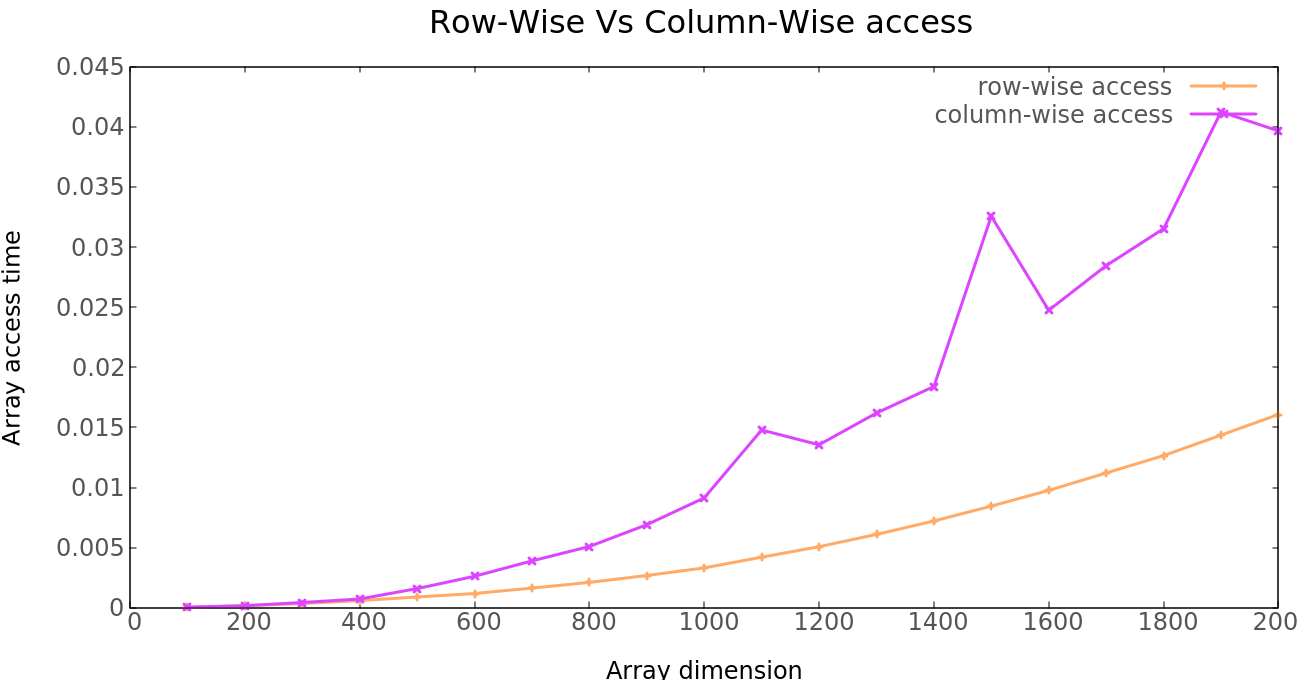
\includegraphics[width=1.00\textwidth]{line-point2.png}
		\end{center}		
		\caption{Line plot of array dimension vs access time, comparing row-wise and column-wise access}
	\end{figure}

	It can be seen that for different array dimensions, accessing/setting data row-wise generally performs better compared to column-wise. \\ \par
	This performance difference can be explained by the way that multi-dimensional arrays are stored and by how instructions are executed in von Neumann model machines \\ \par
	In memory, a two-dimensional array is represented as a block of addresses pointing to the blocks of actual data. This implies that, although each row is stored in a continuous block of memory, the entire array may not be. \\ \par
	This implies that accessing multi-dimensional row-wise takes advantage of sequential locality\footnote{spatial locality when data elements are arranged and accessed linearly}, improving performance over column-wise access.
	\pagebreak
	
	\section{Display output from threads}
	
	After compiling lab12.cpp and running it multiple times, it was noted that the output varied with each execution. The order in which each thread executed was unpredictable and one thread would occasionally execute inbetween another. \\ \par
	This is because a threads execution is controlled by the scheduler. Based on the state of the machine, the scheduler will "decide" which thread to let execute. This causes a generally unpredicatble output. At the same time, since the instructions that the threads are executing are not atomic, the schedule may decide to interrupt a thread and allow another to execute, which may produce "inconsistant" output.

\end{document}
